
\chapter{The role of trust in knowledge based communities} % Main chapter title
\label{Ch:Trust}

%Information and communications technologies (ICTs) have enabled faster and easier creation and sharing of knowledge. Furthermore, they have provided access to a large amount of data which enabled a detailed study of their emergence and evolution \cite{dankulov2015dynamics}, as well as user's roles \cite{saxena2021users}, patterns of their activity \cite{santos2019activity, slag2015one, chhabra2020activity}. 
%However, relatively small attention was given to sustainability of SE communities. Most of the research was focused on the activity and factors that influence the increase of the users’ activity in these communities. Factors such as need for experts and the quality of their contributions have been thoroughly investigated \cite{dev2018size}. It was shown that growth of communities and mechanisms that drive it may depend on the topic around which the community was created \cite{santos2019self}.

The \textbf{Stack Exchange} (SE) is a network of question-answer websites on diverse topics. In the beginning, the focus was on computer programming questions with StackOverflow \footnote{
	More information about StackOverlflow is available at: \url{https://stackoverflow.co/} and broad introduction to SE network is available at: \url{https://stackexchange.com/tour}. 
}  community. Its popularity led to the creation of the Stack Exchange network that these days counts more than 100 communities on different topics. The SE communities are self-moderating, and the questions and answers can be voted, allowing users to earn Stack Exchange reputation and privileges on the site. 

The new site topics are proposed through site Area51 \footnote{Visit \url{https://area51.stackexchange.com/faq} for more details about closed and beta SE communities and the review process.}, and if the community finds them relevant, they are created. Every proposed  StackExchange site needs interested users to commit to the community and contribute by posting questions, answers and comments. After a successful private beta phase site reaches the public beta phase, other members are allowed to join the community. The site can be in the public beta phase for a long time until it meets specific SE evaluation criteria for graduation. Otherwise, it may be closed with a decline in users' activity. However, SE criteria for graduation has not been applied consistently on every SE site, as many sites graduated without reaching all required thresholds. As those measures only quantify the overall number of questions, answers or highly active users, we want to understand how SE community structure evolves and identify factors that influence sustainability. The need to share knowledge with others motivates users to use Q-A platforms. Still, the fact that they interact with each other reveals their sense of belonging to the community and the presence of trust among users. Our proxy for measuring trust in the community is the Dynamic Interaction Based Reputation Model.

We focused analysis on four pairs of SE communities with the same topic. Astronomy, Literature and Economics are active communities \footnote{Astronomy, Literature and Economics graduated on December 2021 and during our research, they were still in the public beta phase.} The first time, these communities were unsuccessful and thus closed. We also compare closed Theoretical Physics with the Physics site, considering that those two topics engage similar type of users. 

\section{Network properties of Stack Exchange data}

On Stack Exchange sites, the interaction between users happens through posts. As we are interested in examining the characteristics of the users, we map interaction data to the networks. Using complex network theory, we can quantify the properties of obtained networks and compare different SE communities, e.g. alive and closed SE sites. 

In the user interaction network, the link between two nodes, user $i$ and $j$, exists if user $i$ answers or comments on the question posted by user $j$, or user $i$ comments on the answer posted by user $j$. The created network is undirected and unweighted, meaning that we do not consider multiply interactions between users or the direction of the interaction. 

First approach is to aggregate all interactions in the first 180 days, and study the properties of static network. Many local and global network measures are dependent 
\cite{boccaletti2006complex}, and it was shown that degree distribution, degree-degree correlations and clustering coefficient are sufficient for description of the properties of complex networks \cite{orsini2015quantifying}. 
 
We calculate the \textbf{degree distribution}, figure \ref{fig:fullnetdeg}, and compare the distributions of active and closed communities of the same topic. Degree distributions between active and closed communities follow similar lines. 
 
 \begin{figure}[ht]
 	\centering
 	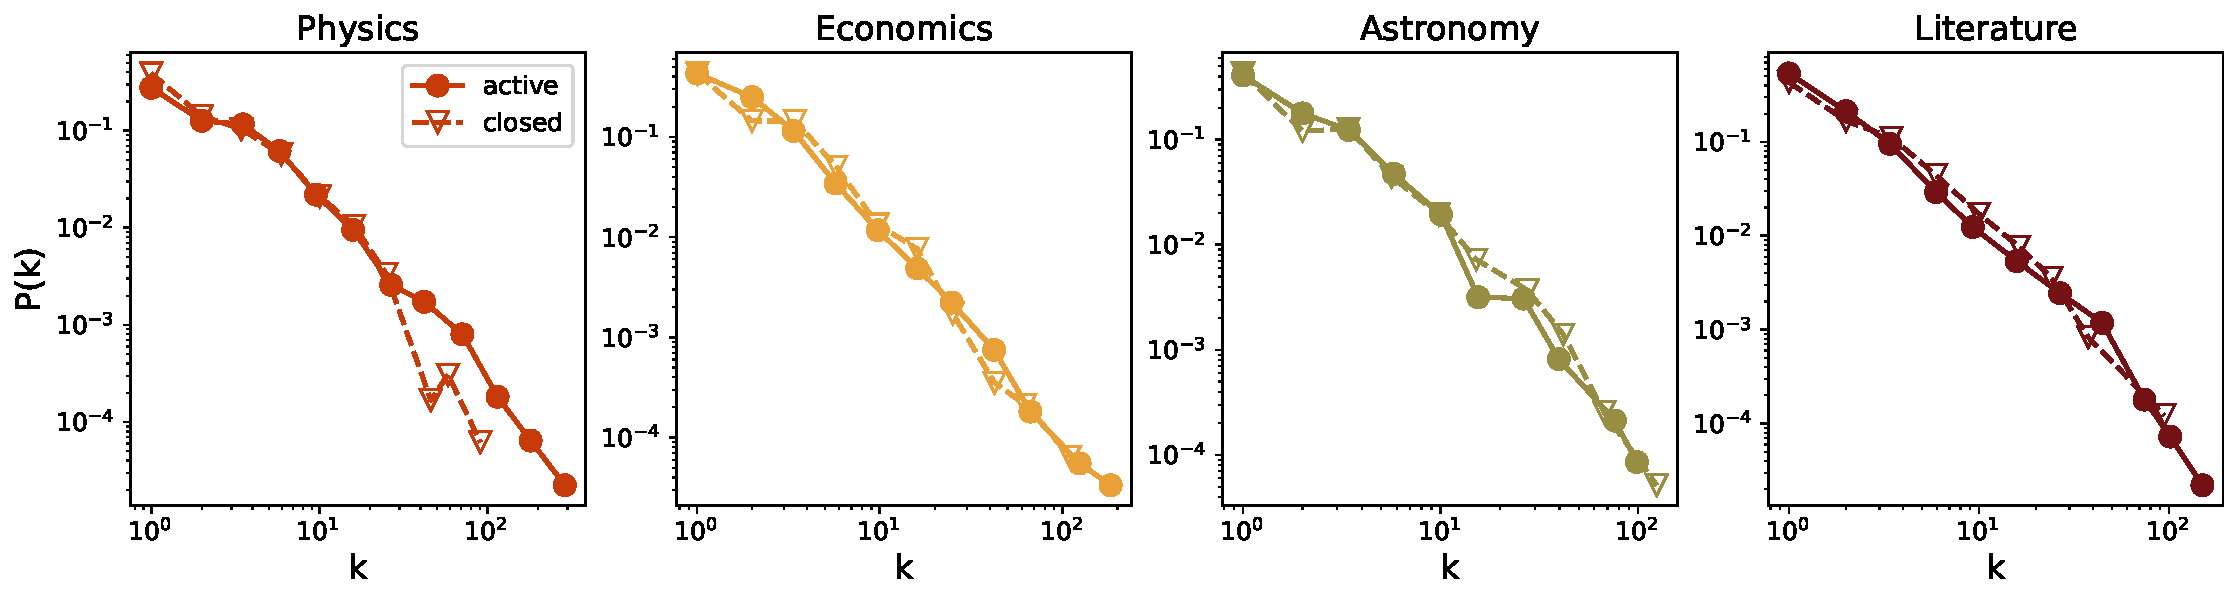
\includegraphics[width=\linewidth]{figures/stackexchange/degree_distribution_fullnet.pdf}
 	\caption{Degree distribution.}
 	\label{fig:fullnetdeg}
 \end{figure}
 
If we take look into \textbf{neighbor degree} dependece on the node degree $k_{nn}(k)$, figure \ref{fig:fullneighdeg} we find that there are structural differences between networks formed in the active and closed communities. On average $k$-degree users in active communities have neighbors with larger degree than it is case in closed communities. The results are consistent for Physics, Economics and Literature. For Astronomy we find different behavior, where the $k_{nn}(k)$ distributions of closed communities are on the top of distributions of the active one. 

\begin{figure}[!ht]
	\centering
	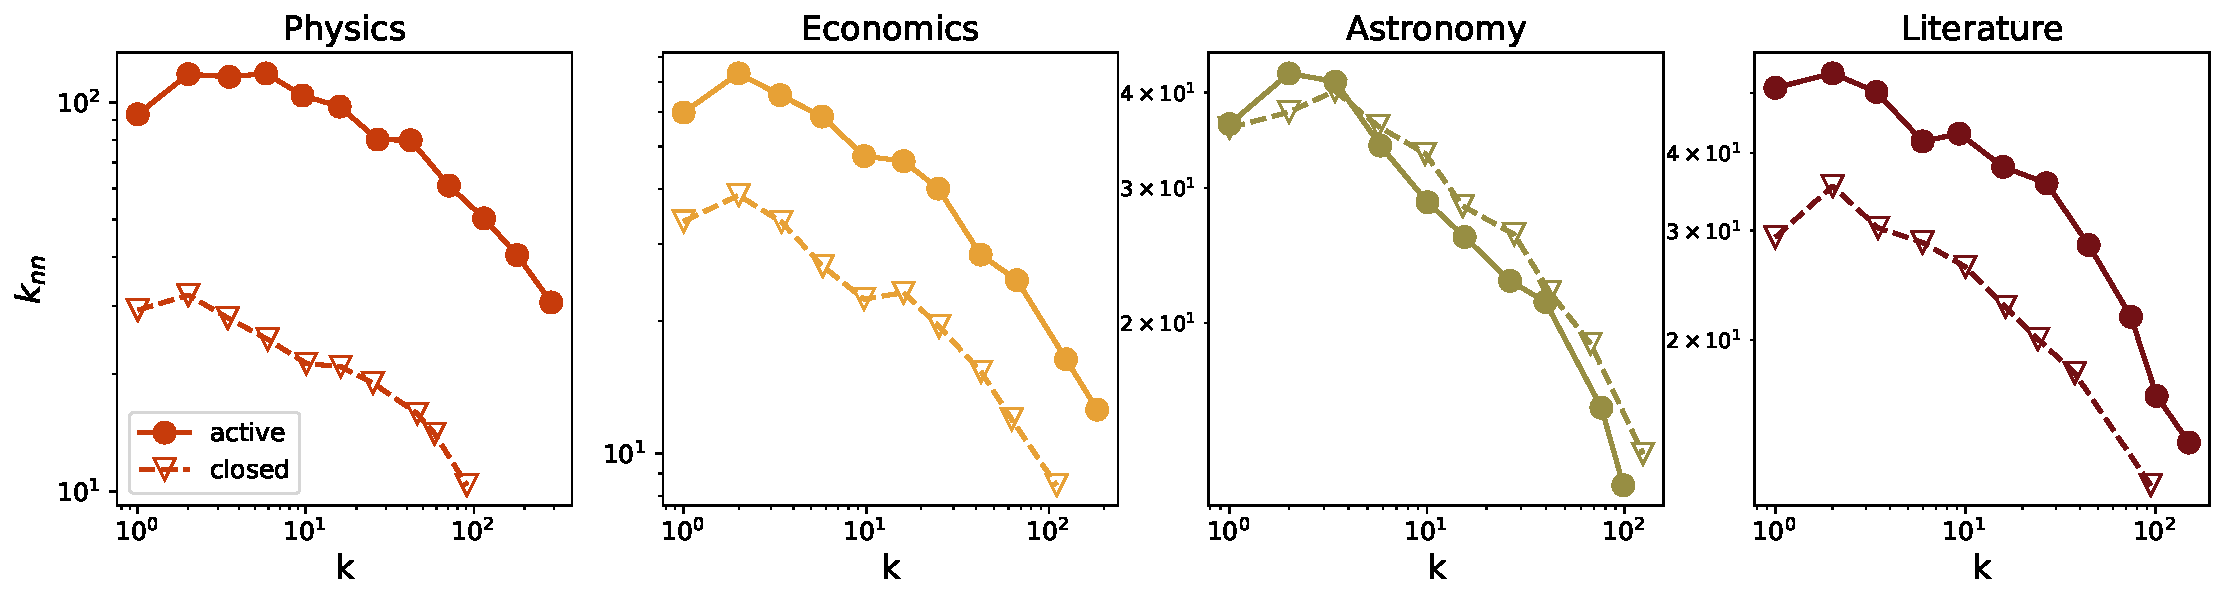
\includegraphics[width=\linewidth]{figures/stackexchange/neighdeg_fullnet.pdf}
	\caption{Neighbour degree.}
	\label{fig:fullneighdeg}
\end{figure}

The \textbf{clustering coefficient} of a node quantifies the average connectivity of between its neighbours and cohesion of its neighborhood \cite{boccaletti2006complex}. It is a probability that two neighbours of a node are also neighbours, and is calculated using the following formula:
\begin{equation}
c_{i}=\frac{e_{i}}{\frac{1}{2}k_{i}(k_{1}-1)} \ .
\label{eq:clust}
\end{equation}
Here $e_{i}$ is the number of links between neighbours of the node $i$ in a network, while $\frac{1}{2}k_{i}(k_{i}-1)$ is the maximal possible number of links determined by the node degree $k_{i}$. The clustering coefficient of network $C$ is the value of clustering averaged over all nodes. Study on dynamics of social group growth shows that that links between one's friends that are members of a social group increase the probability that that individual will join the social group \cite{backstrom2006group}. Furthermore, successful social diffusion  typically occur in networks with high value of clustering coefficient \cite{centola2007cascade}. These results suggest that high local cohesion should be a characteristic of sustainable communities. The dependence of the clustering coefficient on the node degree is shown on figure \ref{fig:fullclustering}. As expected we find that active communities are more clustered.

\begin{figure}[h]
	\centering
	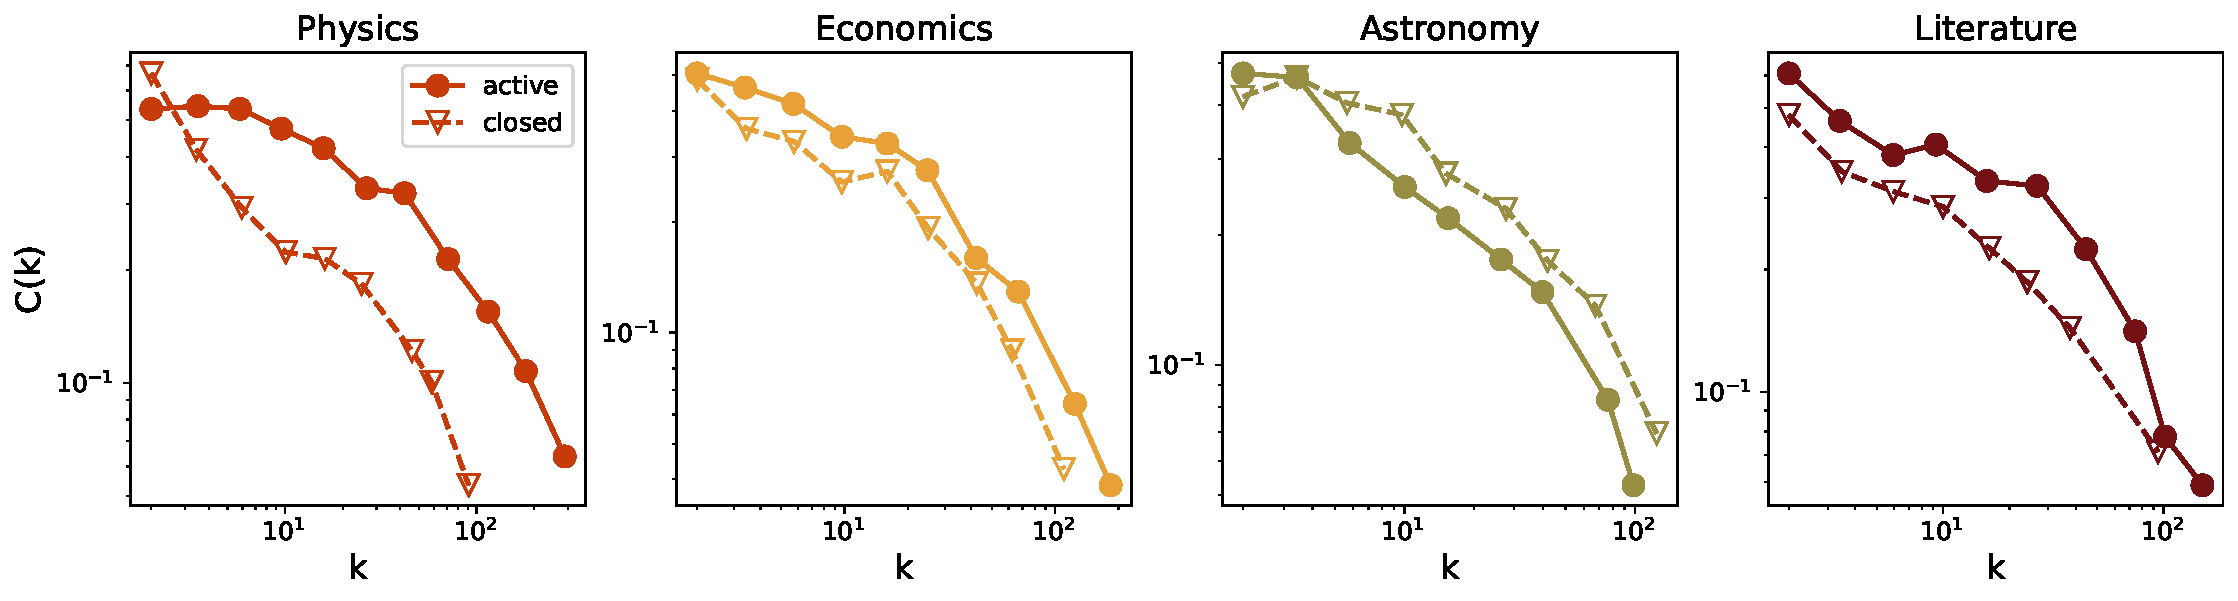
\includegraphics[width=\linewidth]{figures/stackexchange/clustering_fullnet.pdf}
	\caption{Clustering coefficient.}
	\label{fig:fullclustering}
\end{figure}

Instead of creating a static network from the data in the first 180 days of community life, we study how network snapshots evolve. At each time step $t$, we create network snapshot $G(t, t+\tau)$, for time window of the length $\tau$. We fix the time window to $\tau=30$ days and slide it by $t=1$ day through time. Discussion of how the length of the sliding window influences the results is given in appendix A. Sliding the time window by one day, we can capture changes in the network structure daily, as two 30 days consecutive networks overlap significantly. 

Here we investigate how the SE community's clustering coefficient changes with time by calculating its value for all network snapshots. We compare the behaviour of clustering for active and closed communities on the same topic to better understand how the cohesion of these communities is changing over time. Figure \ref{fig:clustering} shows the evolution of the mean clustering coefficient for all eight communities. All communities still alive are clustered, with the value of the mean clustering coefficient higher than 0.1. Physics, the only launched community, has a clustering coefficient value above 0.2 for the first 180 days.

During the larger part of the observed period, an active community's clustering coefficient is higher than its closed pair's clustering coefficient. Let's compare active communities with their closed counterpart. The closed communities have a higher value of the mean clustering coefficient in the early phase, while later communities that are still active have higher clustering coefficient values. These results suggest that all communities have relatively high local cohesiveness and that lower clustering coefficient values in the later phase of community life may indicate its decline. 

\begin{figure}
	\centering
	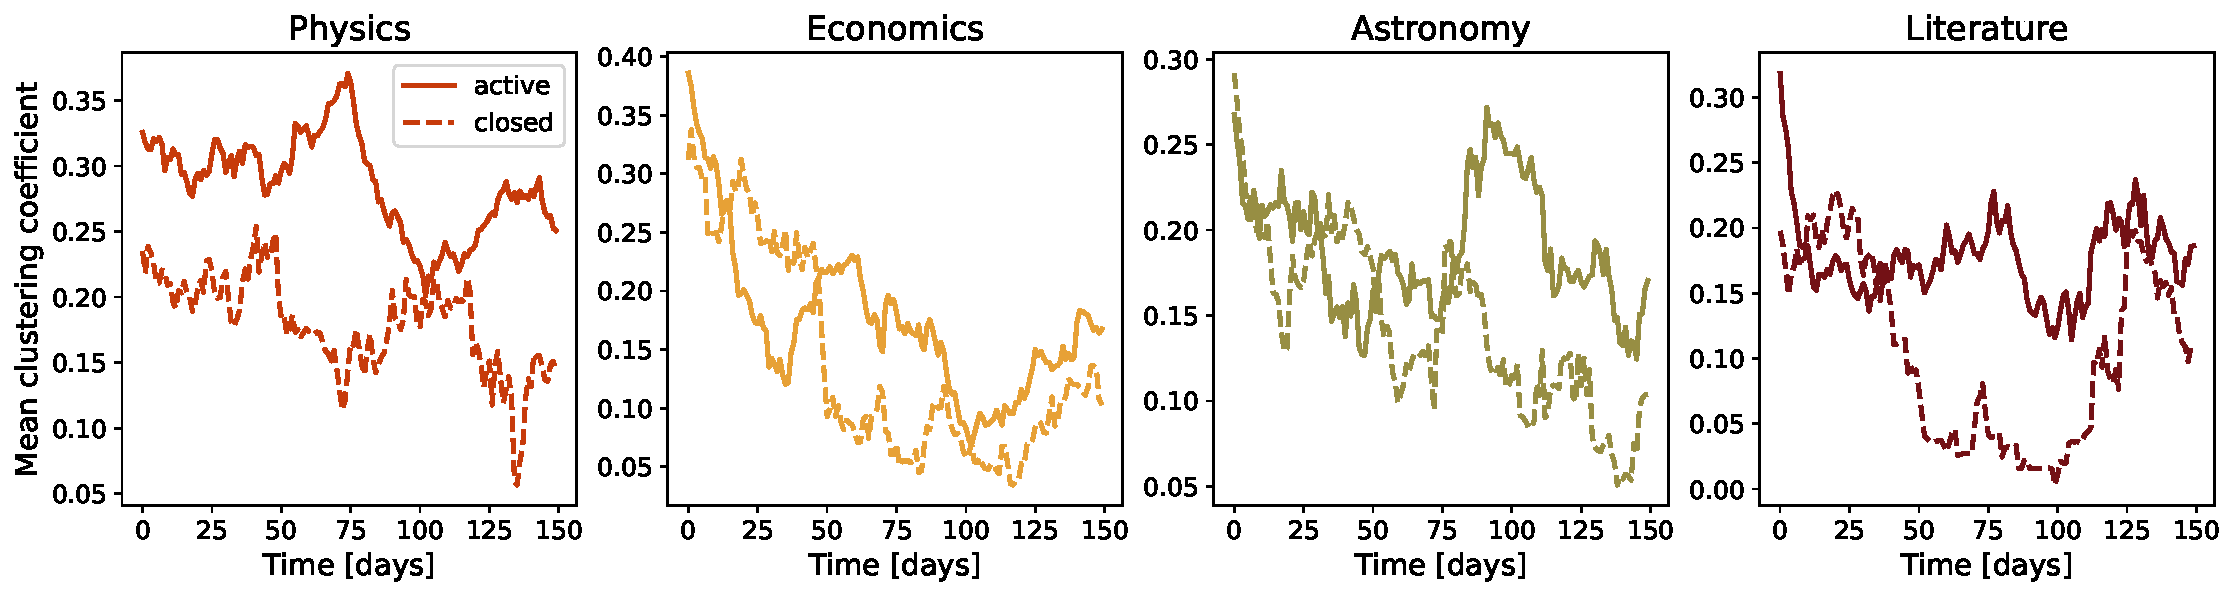
\includegraphics[width=\linewidth]{figures/stackexchange/clustering.pdf}%Figures/figures_SE/Fig3.pdf}
	\caption{Mean clustering coefficient.}
	\label{fig:clustering}
\end{figure}

\section{Core-periphery structure}

Previous research on Stack Exchange communities has attempted to explain how different types of users interact. In Question-Answer communities are expected to be popular and casual users \cite{santos2019activity, santos2019self}. Popular users generate the majority of interactions in the system; they are experts in the community and take care of answering questions and engaging the discussions through comments. As popular users, they considered the $10 \%$ of the most active users and showed that popular users are highly connected with themselves and casual users.

We tested this theory on all eight communities. We focused on 30 days sub-networks and showed how the number of links per node among popular users and between popular and casual users evolves, figure \ref{fig:pop_cas_users}. We also compare active and closed communities of the same topic, so links per node in active sites are more significant than in closed communities.

\begin{figure}[h!]
	\centering
	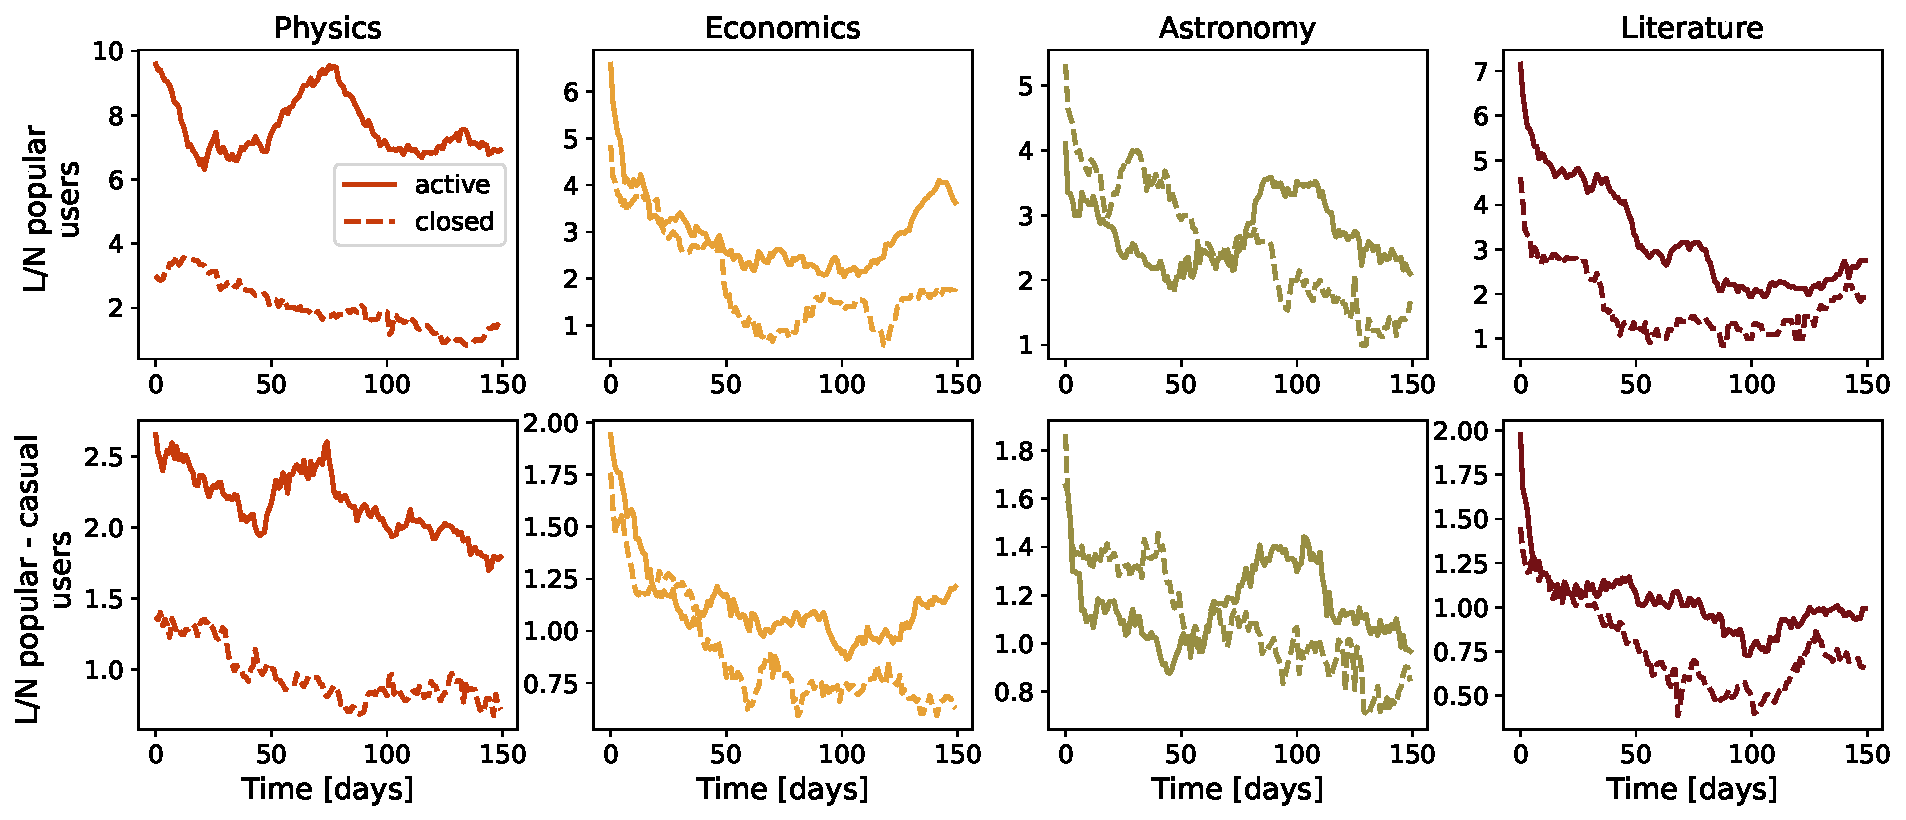
\includegraphics[width=\linewidth]{figures/stackexchange/popular_casual_users.pdf}
	\caption[Number of links per node]{Links per node among popular users (top 10\% of users) and between popular and casual users (everyone but popular users).}
	\label{fig:pop_cas_users}
\end{figure} 

Although we find the difference between active and closed communities, the split according to $10\%$  most active users does not guarantee that all popular users will be considered. Furthermore, the smaller group of frequently active users is similar to the core users in core-periphery structure. This is why we will detect the core of each 30day network. By this, separation is based on the network structure and is more consistent, as using the algorithmic approach, we optimize the connectivity inside the core, periphery and among them. The core-periphery structure has a core that is a densely connected group of nodes, while the periphery has a low density \cite{fortunato2010community, gallagher2020clarified}. 

We use the Stochastic Block Model (SBM) to infer the core-periphery structure of each 30 days network snapshot and analyses how the core structure evolves. The  SBM algorithm is adapted for inferring the core-periphery structure, \cite{gallagher2020clarified}. For each 30 days network, we run the sample of 50 iterations and choose the model parameters according to the minimum description length. As stochastic models start from the random configuration, they can converge to different states, so we analyzed the stability of the inferred structures. More details are given in the appendix. We found that obtained structures differ, but the minimum description length does not fluctuate much. Also, different similarity measures between inferred core configurations take values higher than 0.9, indicating that the core structure is stable. 

The number of users in the core of active communities is higher than in closed communities, the top panel on figure \ref{fig:core_size}. On the other hand, we do not find a big difference between the fraction of core users in the closed and active communities. Furthermore, the fraction of users in core differs from the $10\%$, and it is constantly changing, bottom panel \ref{fig:core_size}. 

\begin{figure}[h!]
	\centering
	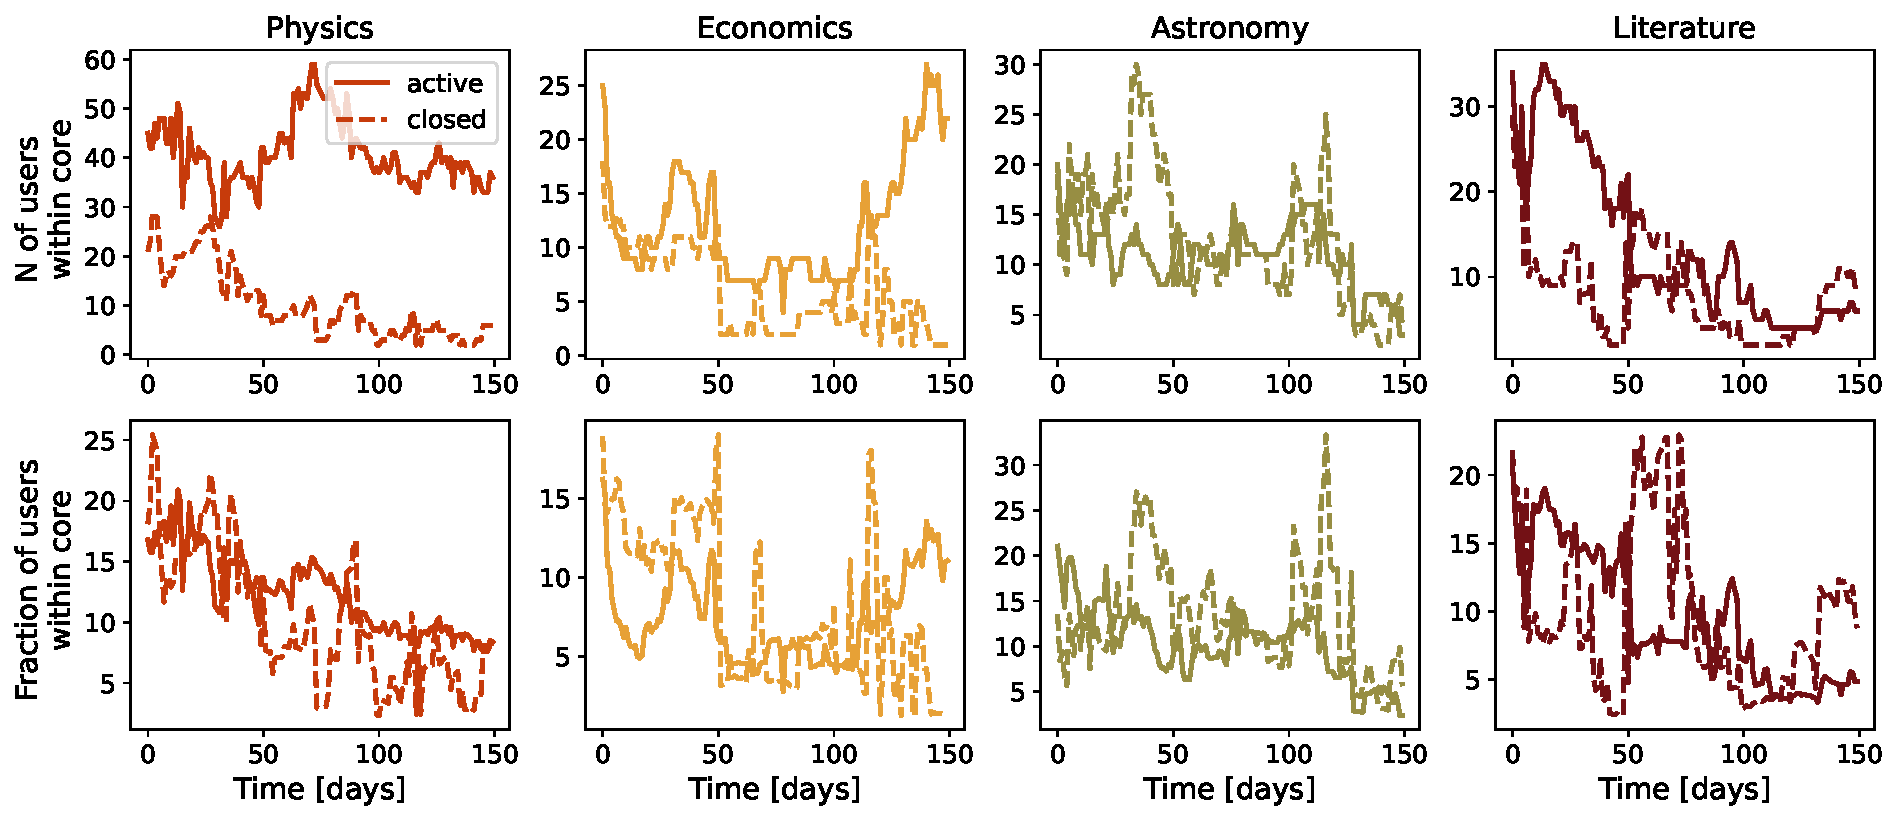
\includegraphics[width=\linewidth]{figures/stackexchange/core_users.pdf}
	\caption[The size of the core]{The size of the core (top) and fraction of users in core (bottom). Solid lines - active sites; dashed lines - closed sites.}
	\label{fig:core_size}
\end{figure}

The number of users is constantly changing. To quantify the stability of the core structure, we compute the Jaccard's coefficient between core users in networks at time points $t_1$ and $t_2$. The Jaccard coefficient range from 0 to 1, so the larger values of the Jaccard index indicate the more similar cores. 
The highest values are found around diagonal elements where we compare networks closer in time, see figure \ref{fig:jaccard_hm}. The core membership changes over time, and the change is more frequent in closed communities. 

\begin{figure}[h!]
	\centering
	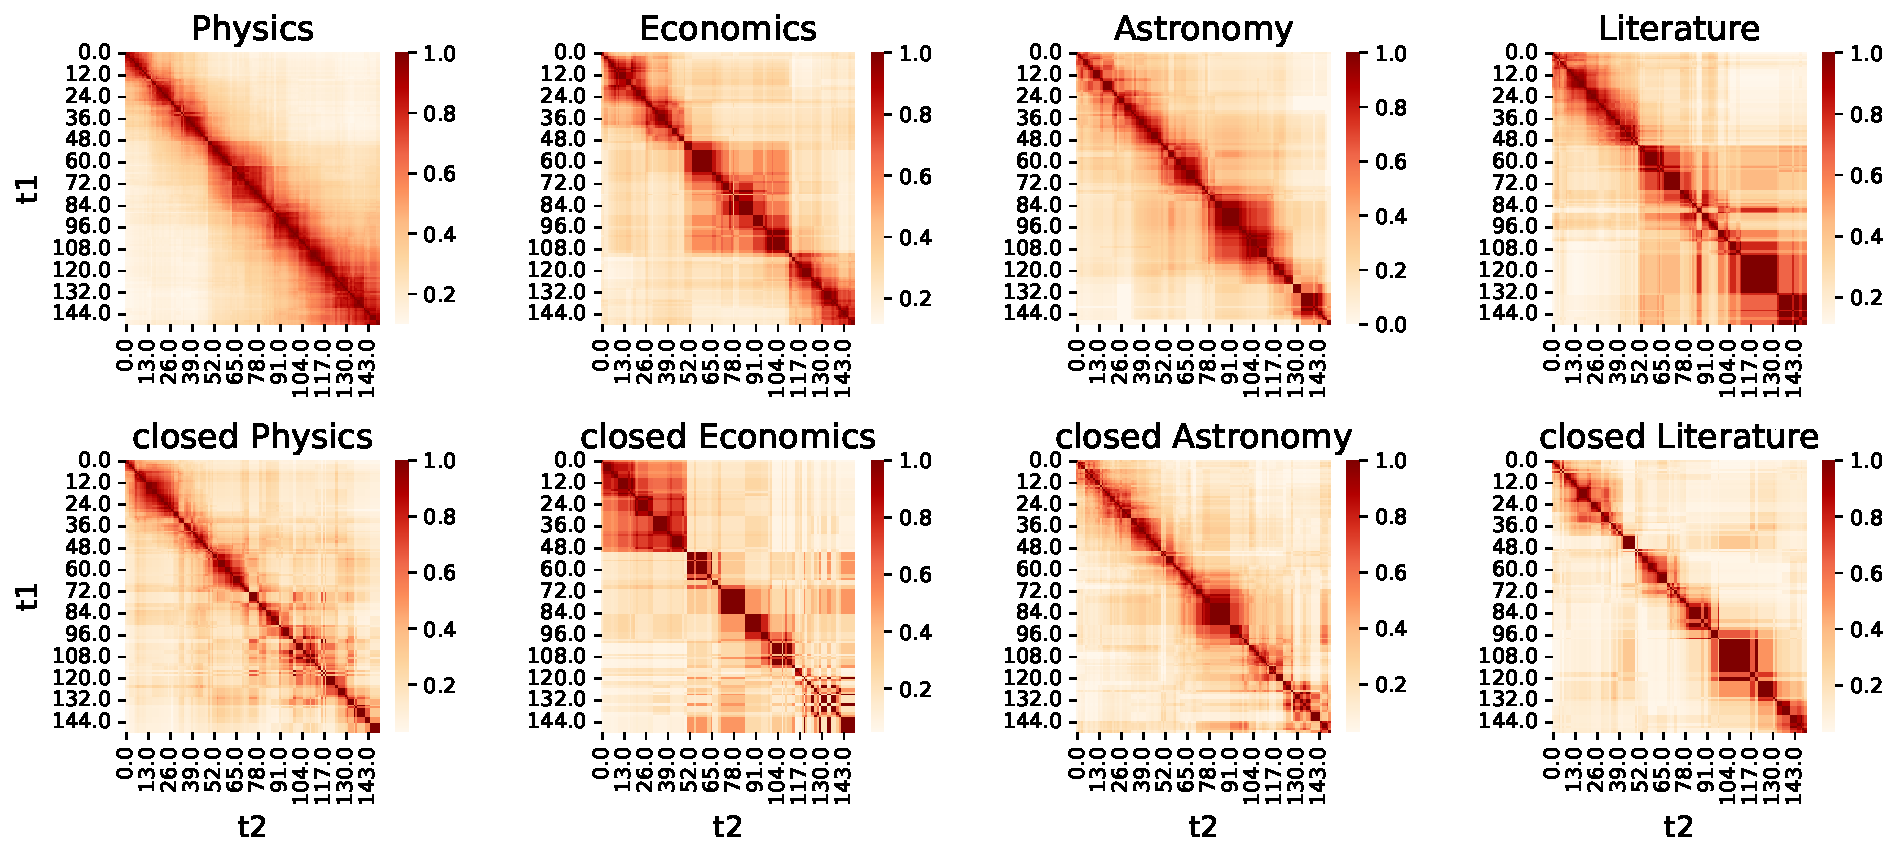
\includegraphics[width=\linewidth]{figures/stackexchange/jaccard_heatmap.pdf}
	\caption[Mean Jaccard index between core users.]{Jaccard index between core users in  sub-networks at time points $t1$ and $t2$.}
	\label{fig:jaccard_hm}
\end{figure}  

The average Jaccard index between cores in networks separated by time interval $t_i-t_j$ with the standard deviation confidence interval are shown in figure \ref{fig:jaccard_mean}. The Jaccard index decreases with the relative time difference between networks faster in closed communities. The relatively high overlap between distant networks confirms that active networks have a more stable core. 

\begin{figure}[h!]
	\centering
	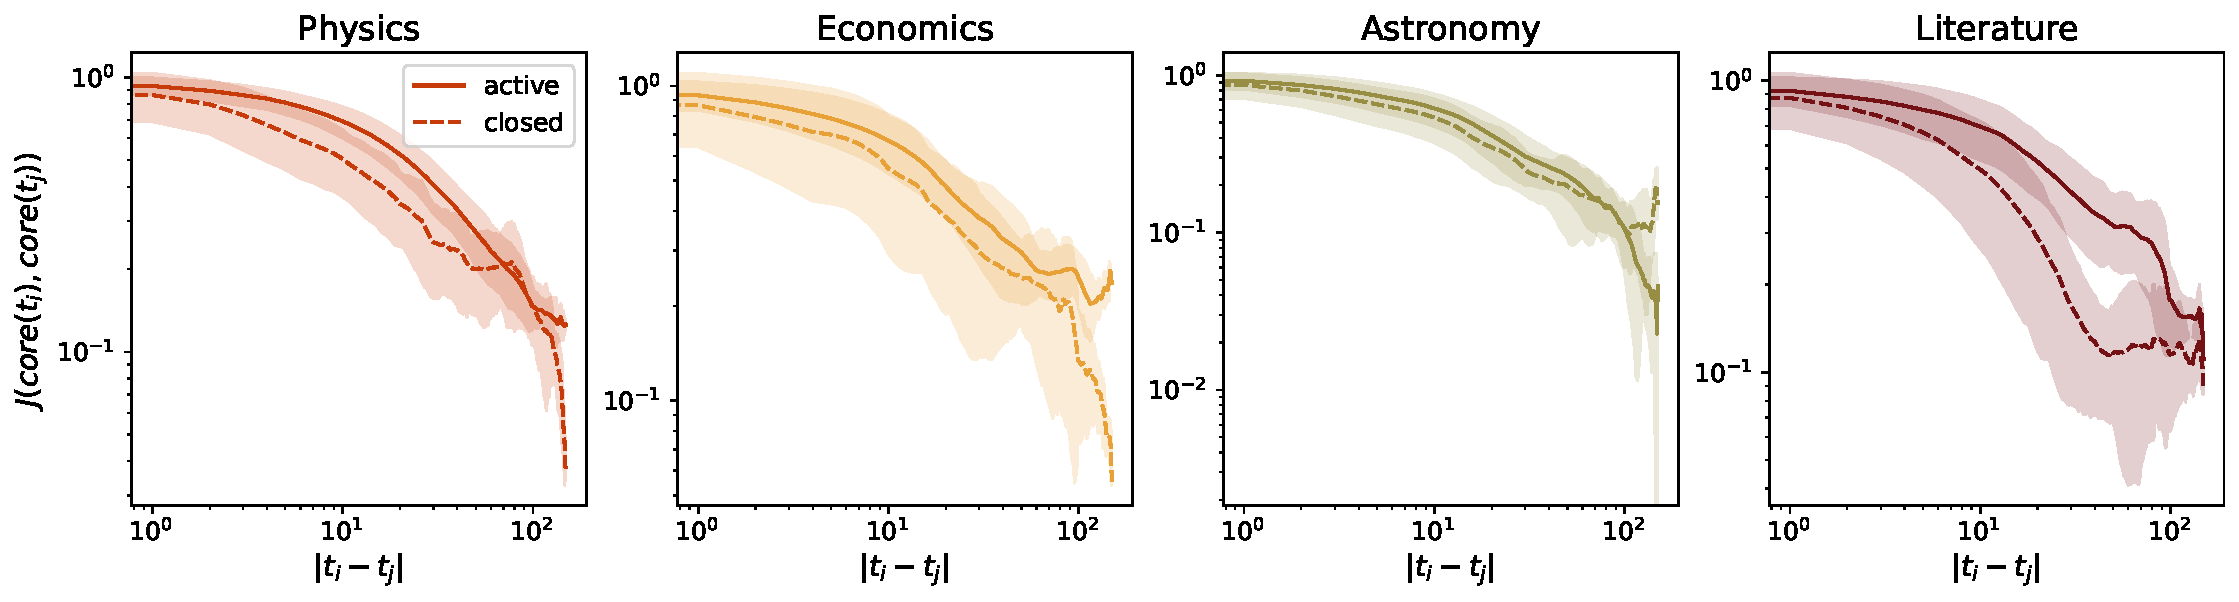
\includegraphics[width=\linewidth]{figures/stackexchange/jaccard.pdf}
	\caption[Mean Jaccard index between core users.]{Jaccard index between core users in 30days sub-networks for all possible pairs of 30 days sub-networks separated by time interval $|t_i - t_j|$.}
	\label{fig:jaccard_mean}
\end{figure}

Finally, we examine how the users' connectivity in and between the core and periphery evolves. In the figure, we show the $L/N$ in the core, which is proportional to the average degree of the network $2L/N$, \ref{fig:links_per_node}. The Physics community has more than twice the connectivity than closed Theoretical Physics. For Literature, we also find higher connectivity. Still, at the end of the observation period, the connectivity in the active site drops and becomes similar as in the closed one. For Economics and Astronomy, the difference between active and closed sites is not so clear. At the beginning of the period for the sites on the economic topic, connectivity is similar. After 50 days of community life, connectivity in active communities is starting to rise, while in the case of closed economics, it is dropping. For Astronomy, the connectivity is higher in closed communities, in the first 50 days. After this period, we find a sudden rise in the connectivity of active astronomy, but again it drops and becomes comparable to the connectivity values in the closed site. Similar conclusions can be drawn for the connectivity between core and periphery. The largest difference between active and closed sites is observed in Physics.  

\begin{figure}[h]
	\centering
	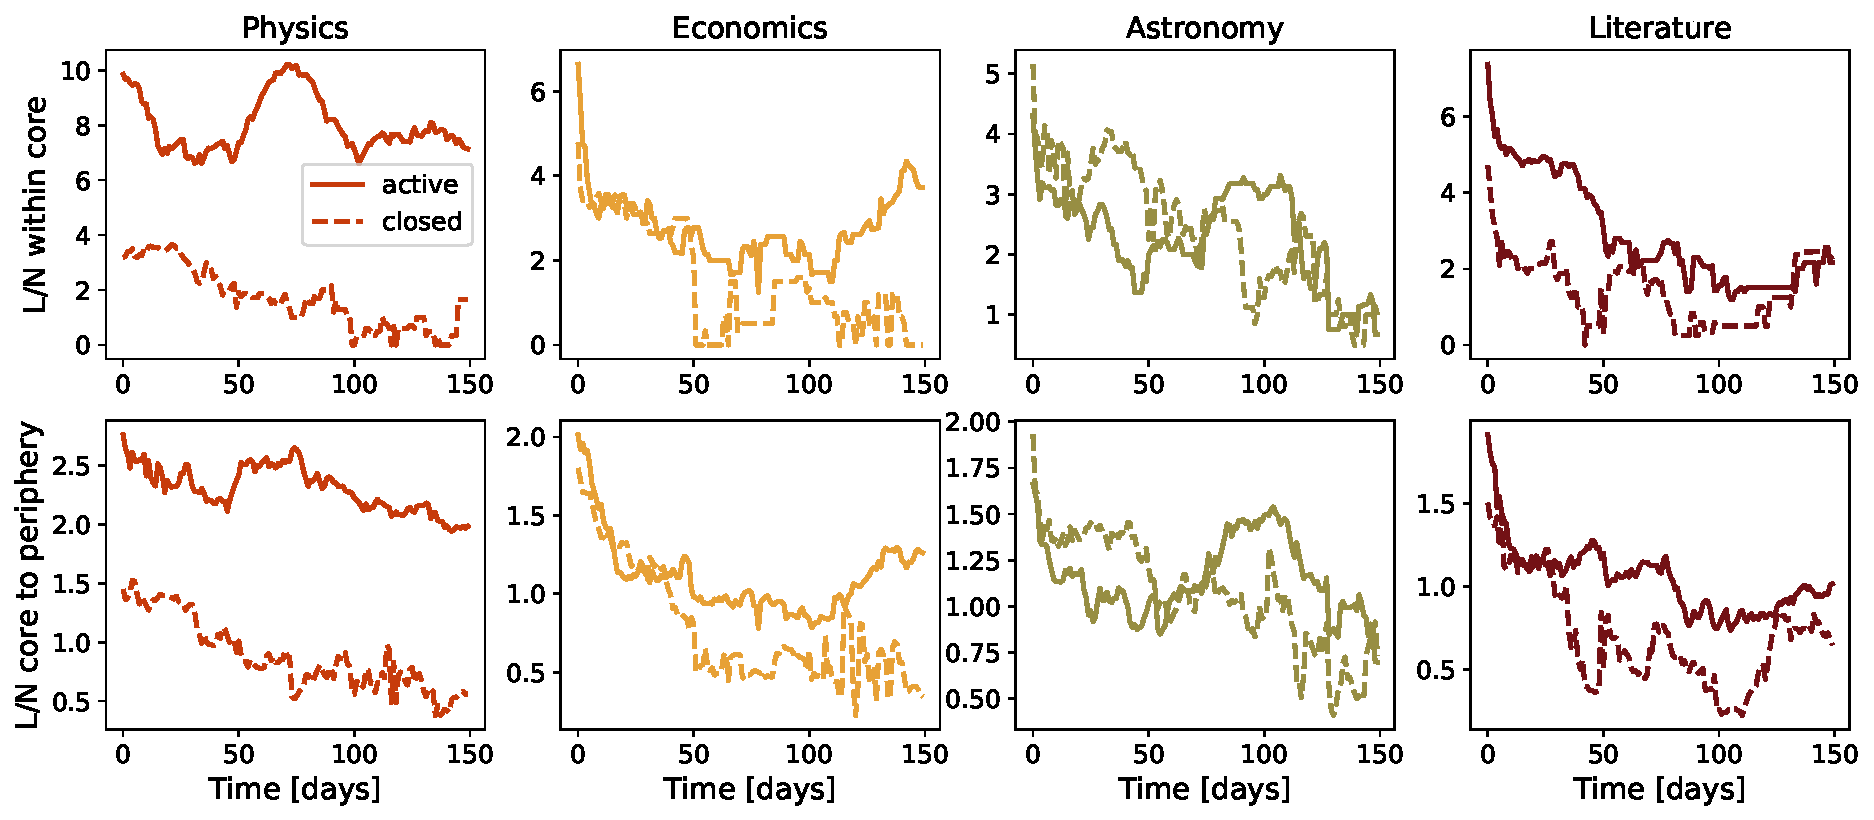
\includegraphics[width=\linewidth]{figures/stackexchange/core_connectivity.pdf}
	\caption{Links per node in core and links per node between core and periphery.}
	\label{fig:links_per_node}
\end{figure}

\section{Dynamical Reputation on Stack Exchange communities}

We further explore the difference between active and closed communities through the dynamical reputation model. With this model we calculate the reputation of each user in the community. The reputation is directly connected with the collective trust in the network. 

\begin{figure}[h]
	\centering
	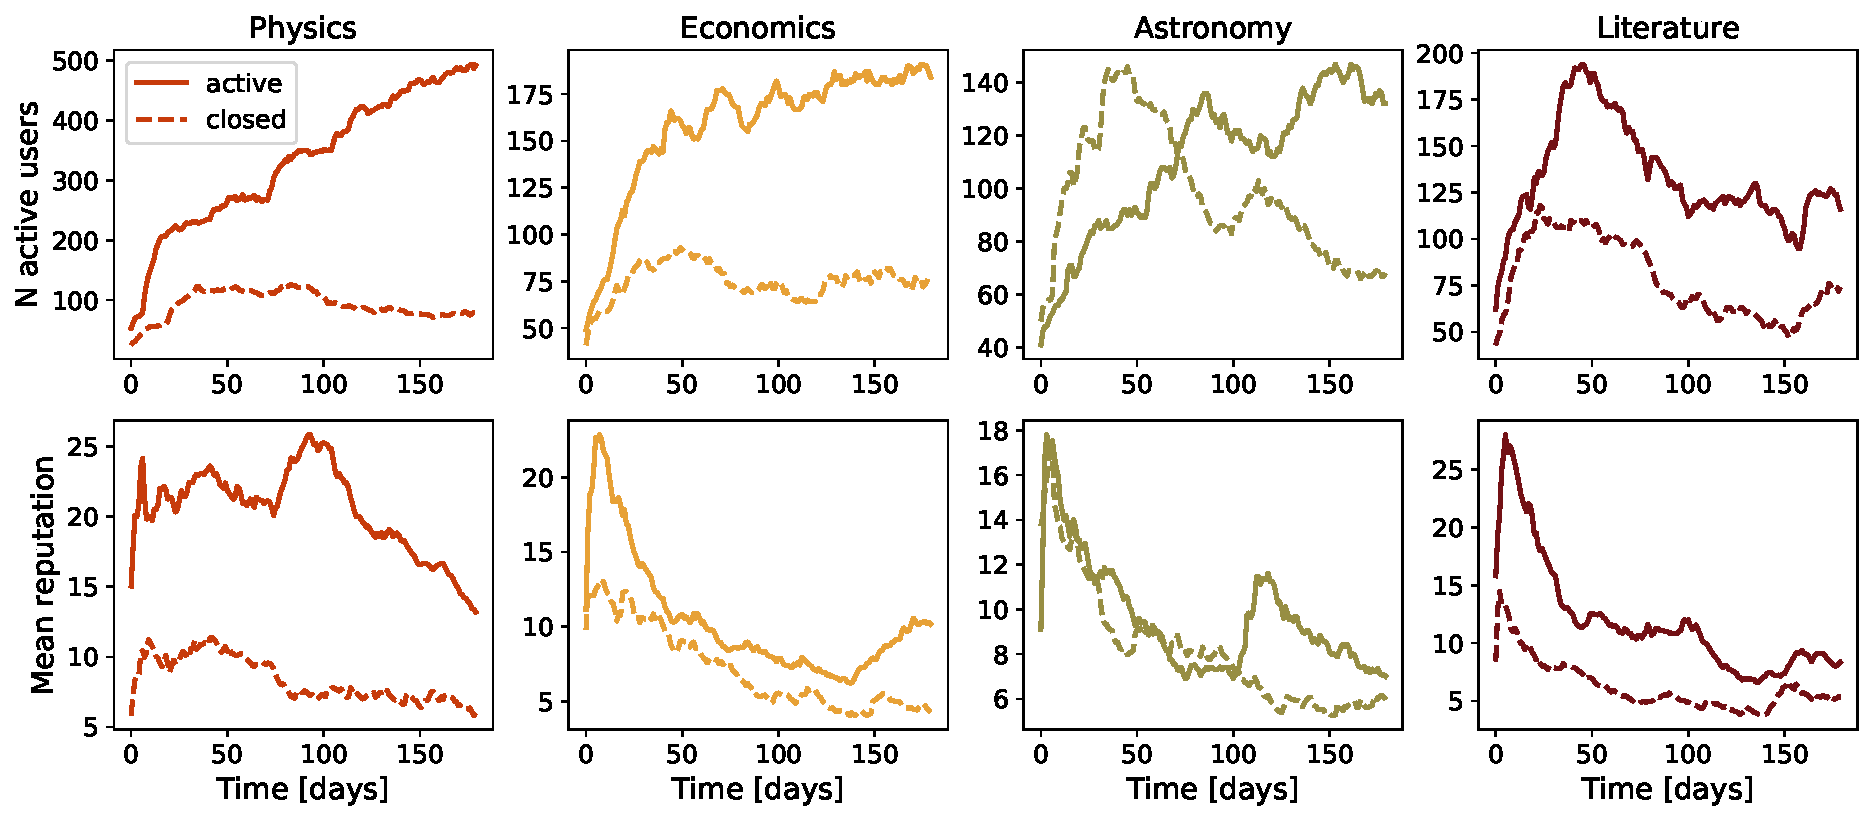
\includegraphics[width=\linewidth]{figures/stackexchange/reputation.pdf}
	\caption[Dynamic Reputation of Stack Exchange websites.]{Dynamic Reputation on the four pairs of Stack Exchange websites: Astronomy, Literature, Economics,  Physics and Theoretical Physics.}
	\label{fig:dr6panel}
\end{figure}

Dynamical reputation model, introduced in section \ref{sec:met_dibrm} has three parameters. We explored different parameter combinations to find the set of parameters the most suitable for a given system of Stack Exchange communities. First, the basic reputation is set to $I_{bn}=1$. The cumulative factor is $\alpha=2$, as we want to emphasize the frequent interactions. The parameter $\beta$ controls the reputation decay due to user inactivity. After the last activity, for some period, the user has a positive reputation and is still impacting the other users. We optimized the number of users with a reputation larger than $1$ according to the number of users in the 30 days network, and concluded that parameter $\beta=0.96$. A more detailed discussion about the choice of the parameters is in the appendix. 

With selected model parameters, we calculated the reputation of each user. If a user has a reputation larger than $1$, it is considered active, but when the reputation drops below this threshold means that the user has not been active long enough; it does not make a valuable contribution to the community. The number of active users and their mean reputation for different SE sites are shown in figure \ref{fig:dr6panel}. 

From the properties of networks, we found that active communities are more cohesive and have a more stable core. Furthermore, we focus our analysis on the dynamic reputation of the core users. Figure \ref{fig:dr_core} shows the evolution of mean user reputation within the core. Active communities have a larger reputation than their closed counterpart. As it is previously suggested, the largest difference is found in the Physics community. For other communities, the difference is not so striking, still, on average the core of active communities has a larger reputation than the core of closed communities. 

\begin{figure}[h]
	\centering
	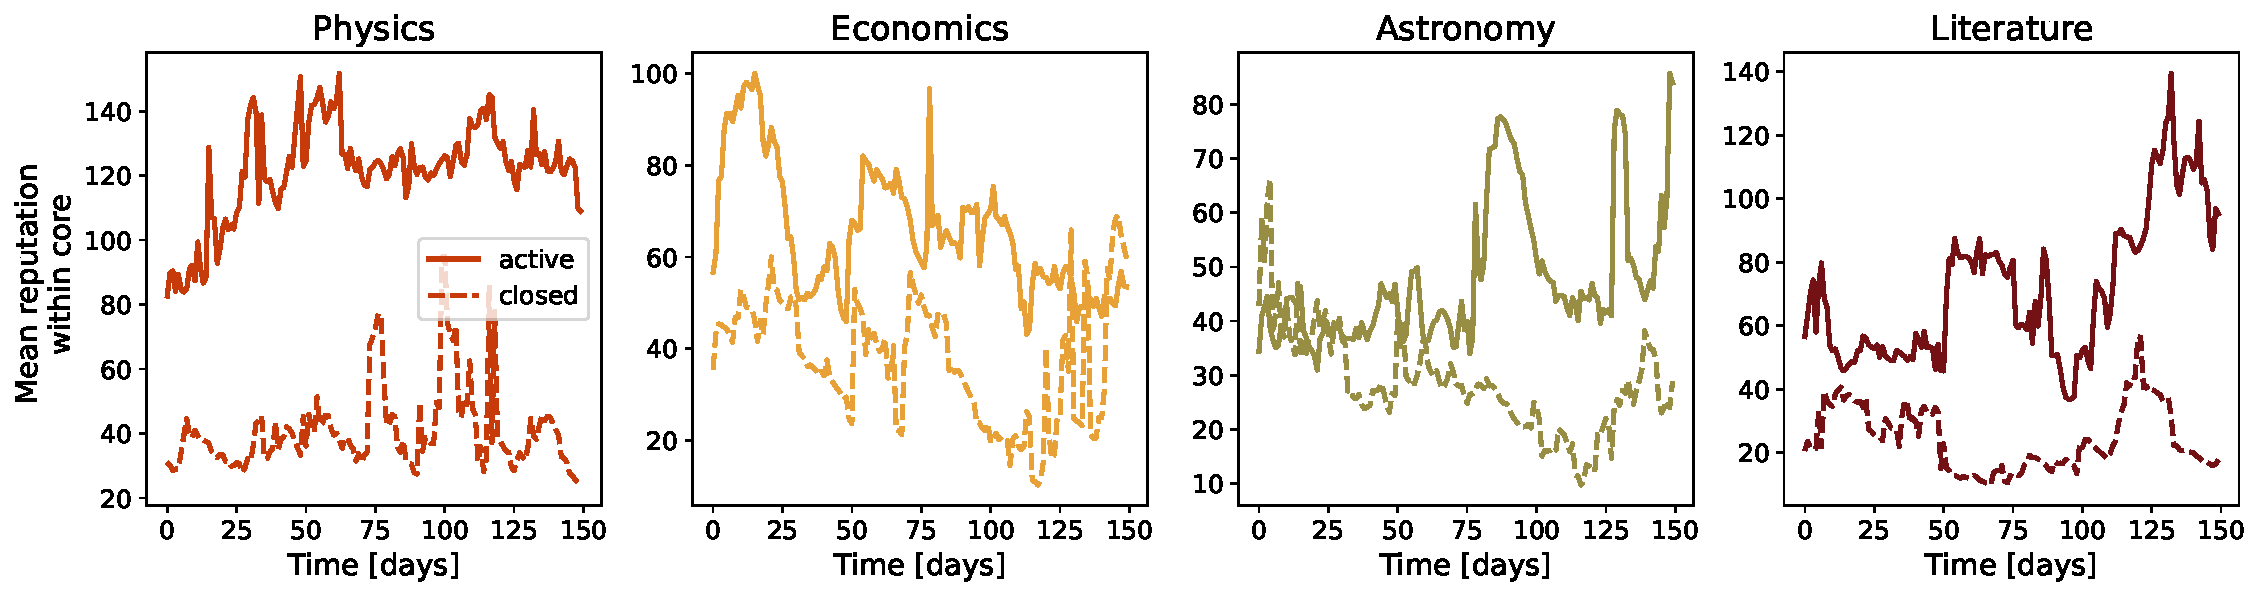
\includegraphics[width=\linewidth]{figures/stackexchange/core_reputation.pdf}
	\caption{Dynamical reputation within core.}
	\label{fig:dr_core}
\end{figure}

In the core of the network are very active users, and we expect a higher dynamical reputation compared to the total reputation of users belonging to the periphery. The ratio between core and periphery in Physics is always higher than in Theoretical Physics, and similar conclusions are observed for the literature. In the early days of Economics, we find a different pattern; the core-periphery reputation ratio is larger for closed Economics, but later it changes in favour of active Economics. Astronomy shows different behaviour where the closed community where dominantly; closed astronomy had a larger core-periphery reputation ratio. 

\begin{figure}[h!]
	\centering
	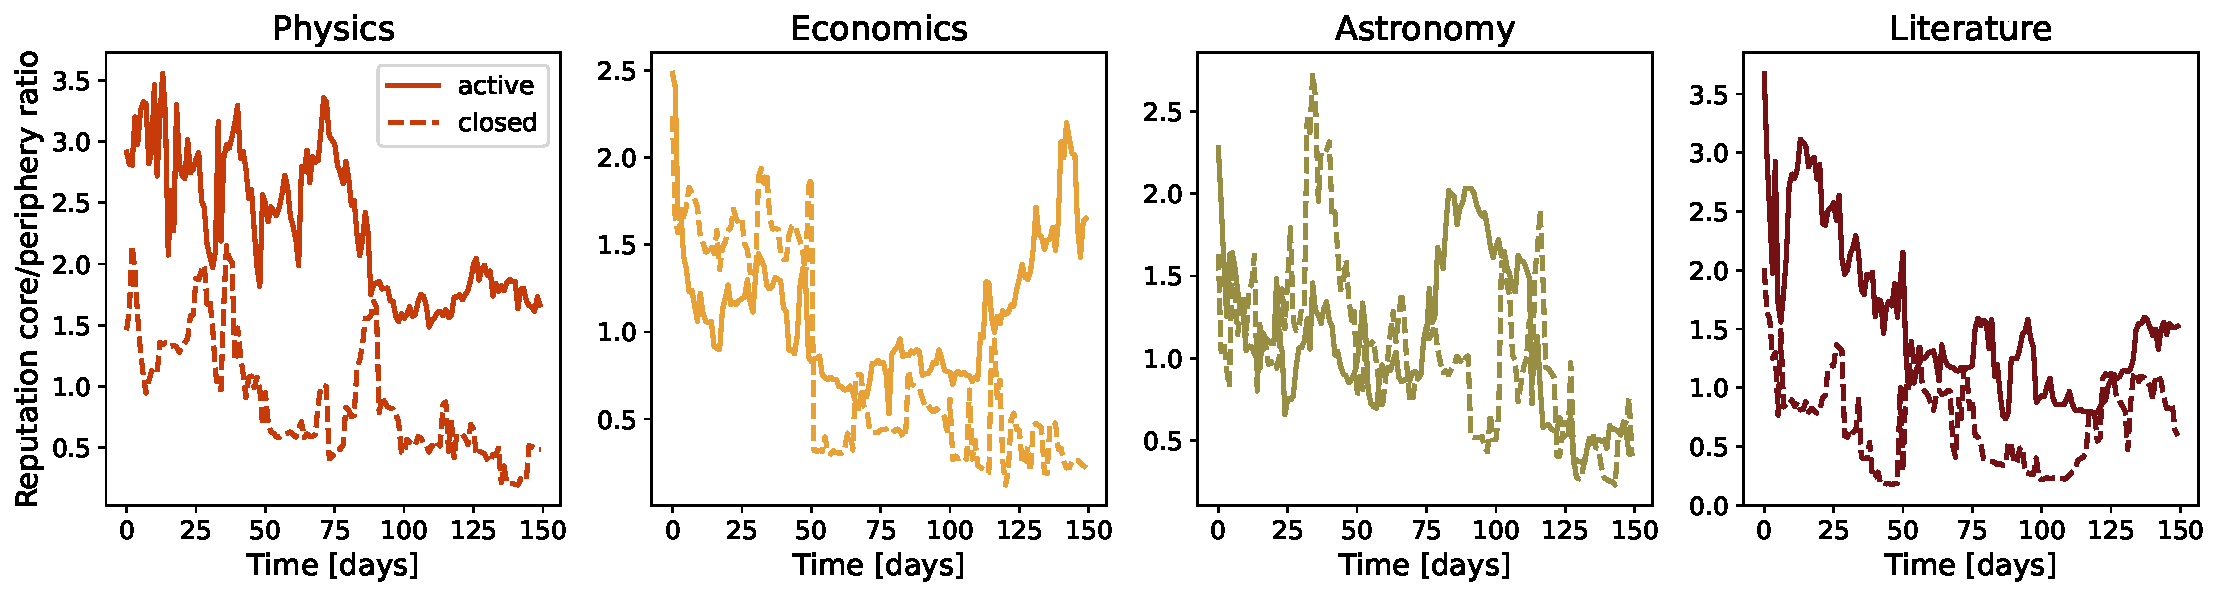
\includegraphics[width=\linewidth]{figures/stackexchange/core_per_ratio_reputation.pdf}
	\caption[Ratio between the total reputation within network core and periphery.]{Ratio between the total reputation within network core and periphery. Solid lines active communities, dashed lines closed communities.}
	\label{fig:dr_core_per}
\end{figure}

The distribution of the dynamic reputation of SE communities are skewed. We calculated the Gini coefficient to better express the difference between distribution reputations. This measure quantifies the inequality among users' reputations. The Gini coefficient is calculated based on reputation values for each day; see figure \ref{fig:dynrep-gini}. The Gini coefficient is larger than $0.5$, in the first 180 days. Also, the active communities showed more reputation inequality and dynamical reputation has larger variation. 

\begin{figure}[h]
	\centering
	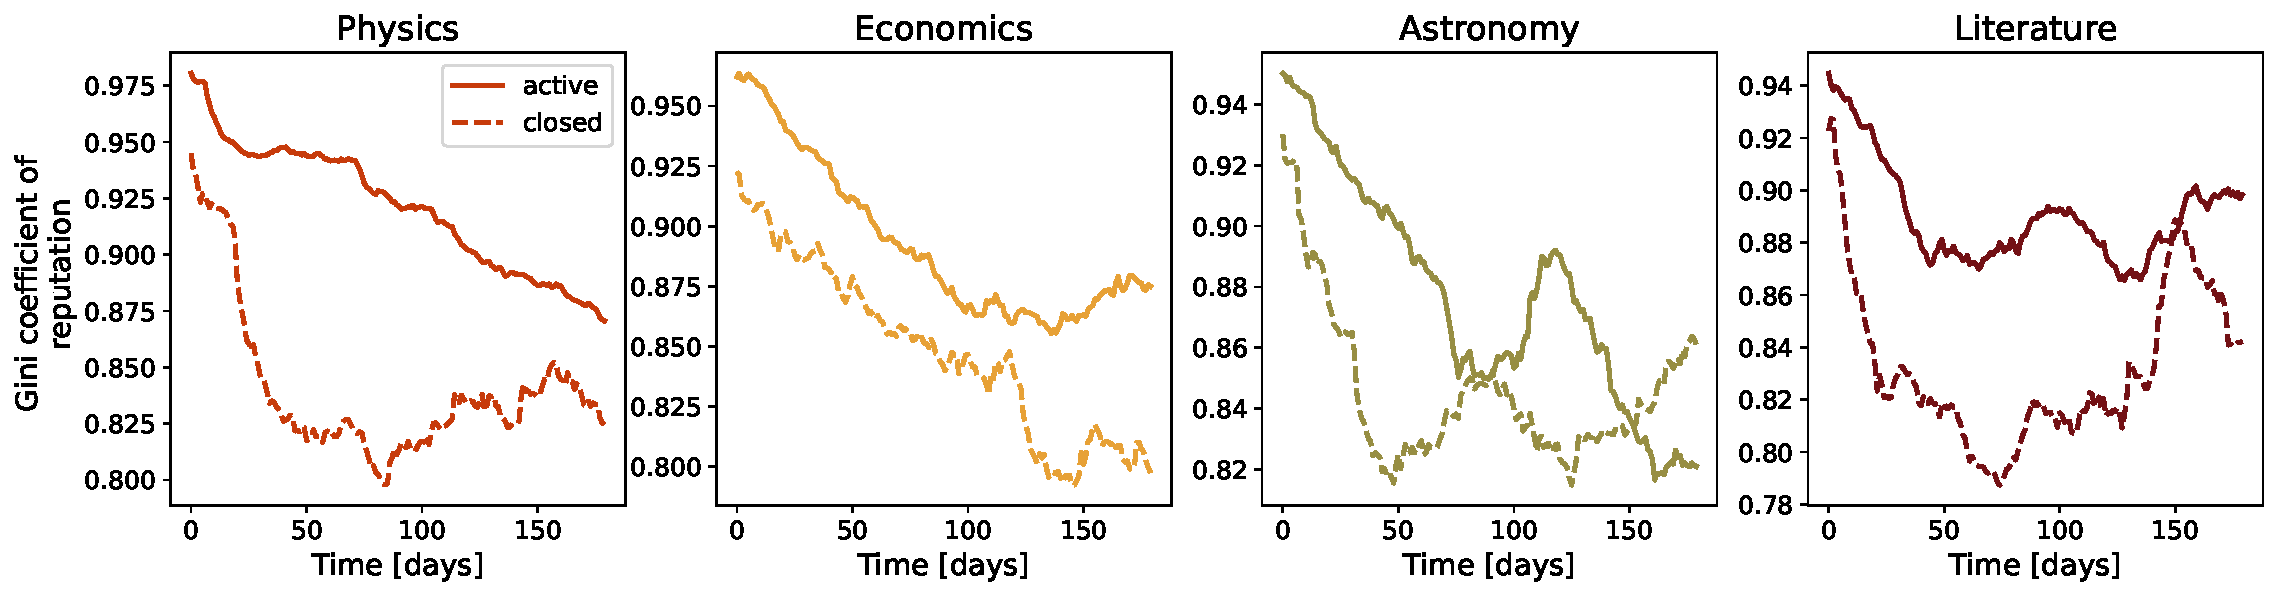
\includegraphics[width=1\linewidth]{figures/stackexchange/gini.pdf}
	\caption[Gini index of dynamic reputation]{Gini index of dynamic reputation within population.}
	\label{fig:dynrep-gini}
\end{figure} 

Further, we investigate how the properties of user interaction networks correlate with the user's reputation. For example, we can measure the assortativity coefficient among connected users in the network. For each 30 days user interaction network, we calculate the reputation assortativity, using the reputation value observed on the last day of the time window in which the network is constructed. With this measure, we quantify whether users tend to connect with users with similar reputations or not. Figure \ref{fig:dyn_rep_assort} shows results where we compare each SE community's active and closed sites. Assortativity has small values in all communities' reputations, not larger than $|0.3|$. In active communities, this is a mostly negative measure showing expected user behaviour: popular users, who often have a high dynamical reputation, interact with users with low dynamical reputations. Astronomy is an outlier again; during the first 100 days active community had a positive reputation for assortativity, and after this period, it started behaving similarly to other active communities. 

\begin{figure}[h]
	\centering
	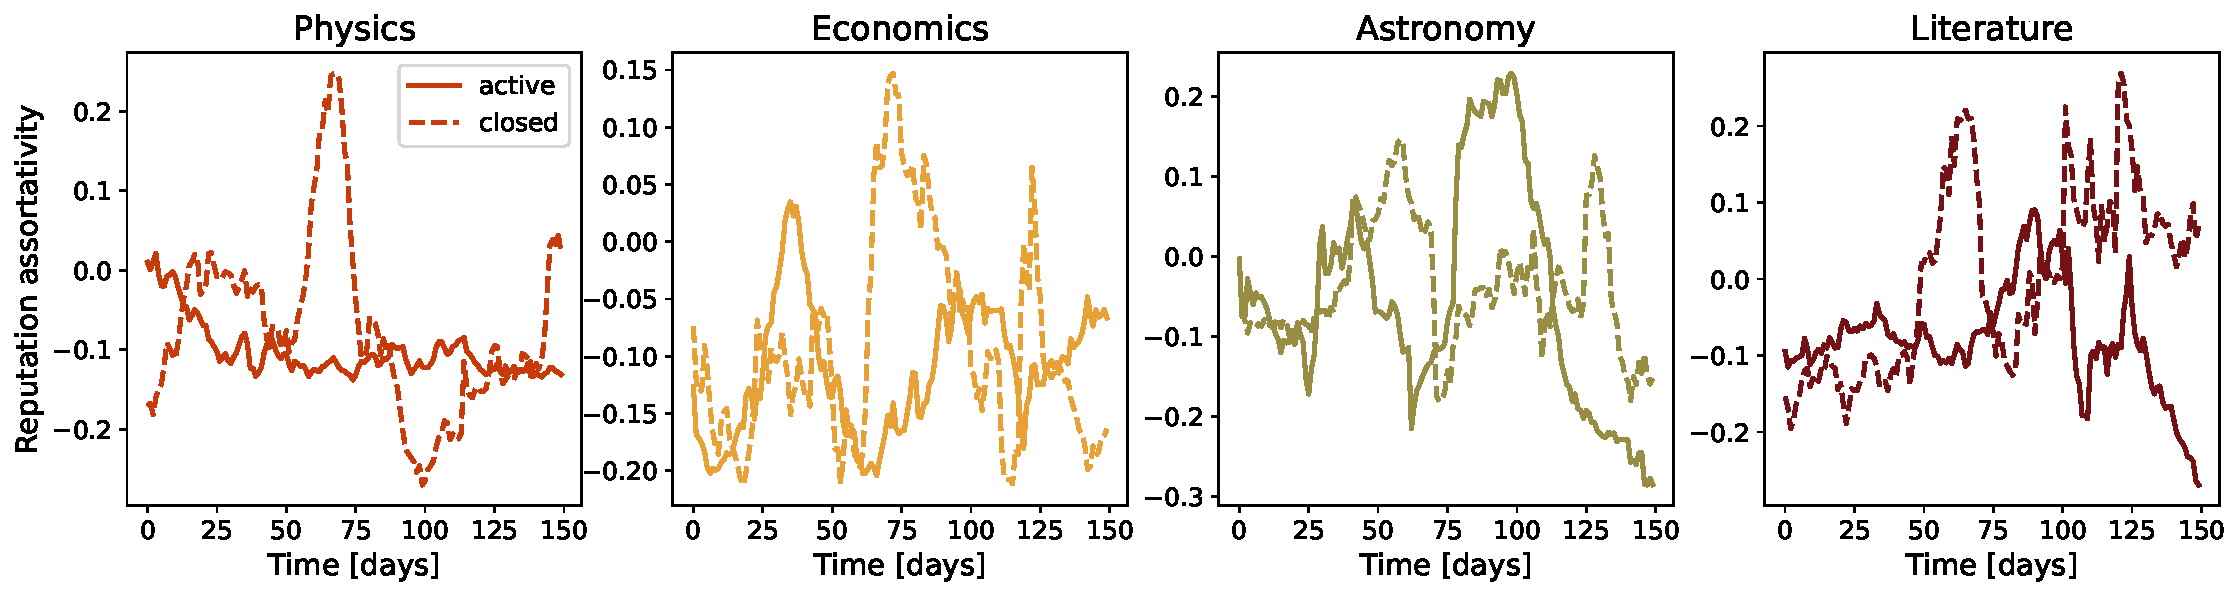
\includegraphics[width=1\linewidth]{figures/stackexchange/reputation_assortativity.pdf}
	\caption[Dynamic Reputation assortativity]{Dynamic Reputation assortativity in the network of interactions (questions, answers, comments, unweighted, undirected network). Solid lines - active sites; dashed lines - closed sites.}
	\label{fig:dyn_rep_assort}
\end{figure}

Finally, we are interested in how dynamical reputation correlates with network measures. We compare the node's centrality in the 30-day network and the node's reputation on the last day of the 30 day sliding window. The correlation coefficient between dynamic reputation and node degree is very high; see top panel on \ref{fig:dyn_rep_centrality}. The bottom panel shows correlations between dynamic reputation and betweenness centrality in the network, which are also high. We find that correlations are mostly higher in active communities; only for astronomy they take similar values during the observed period. 

\begin{figure}[h]
	\centering
	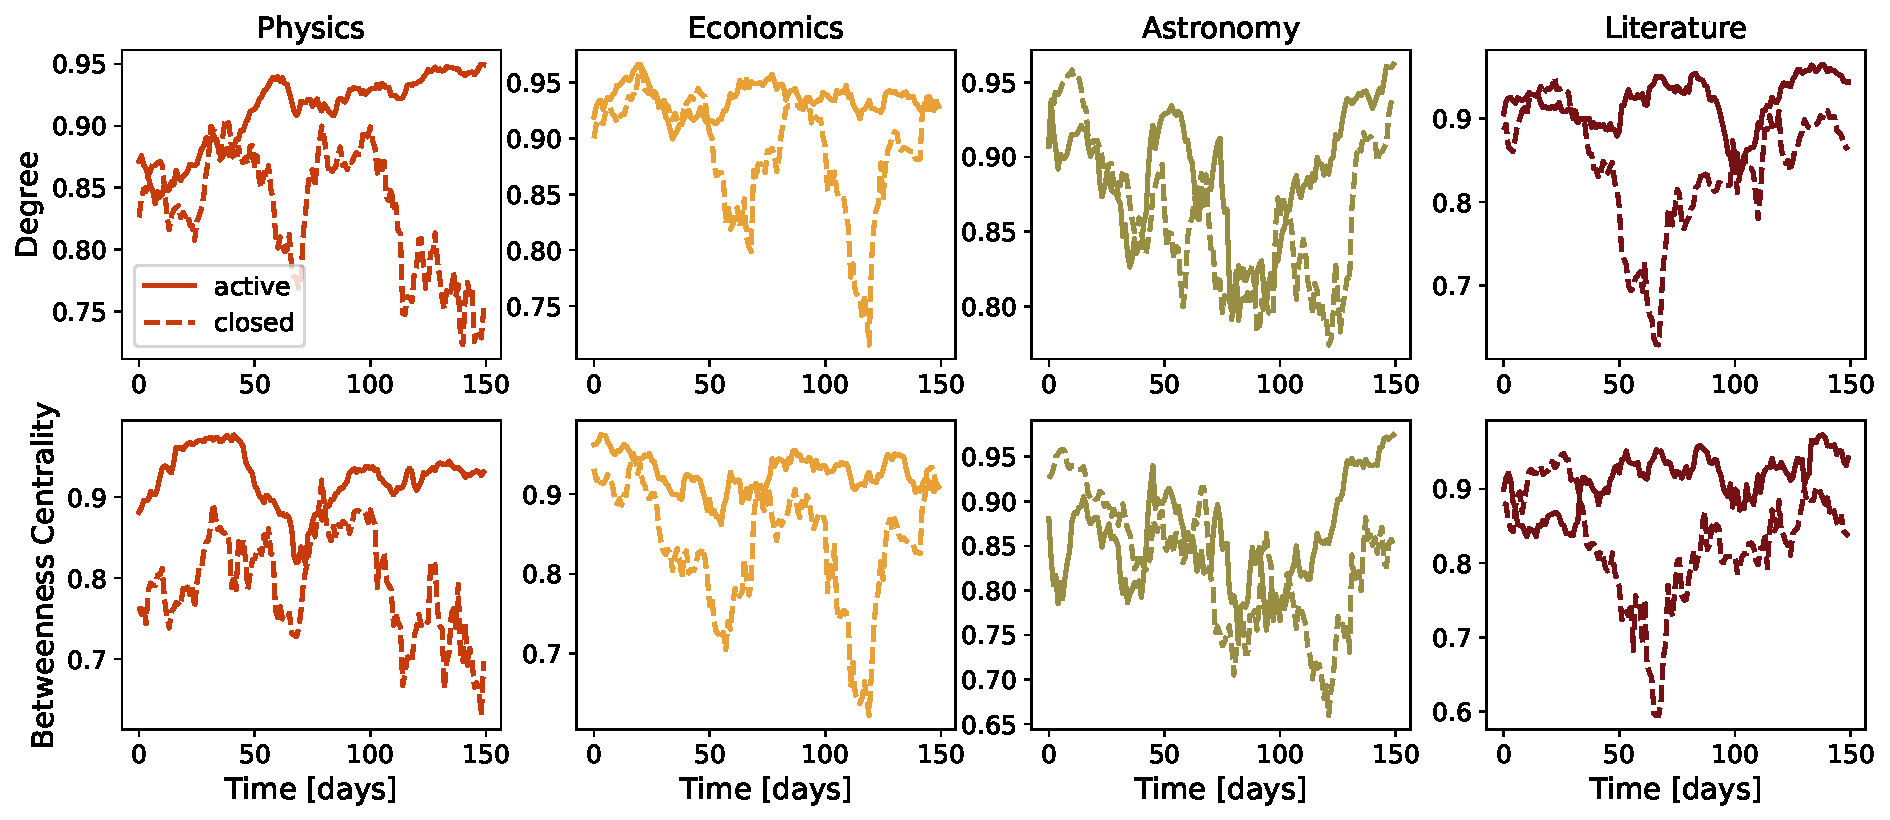
\includegraphics[width=\linewidth]{figures/stackexchange/correlations.pdf}
	\caption[Coefficient correlation between ]{Coefficient of correlation between users' Dynamic Reputation and users' network degree (top) and users's betweenness centrality (bottom). Solid lines - active sites; dashed lines - closed sites.}
	\label{fig:dyn_rep_centrality}
\end{figure}

\section{Conclusions}

The Stack Exchange sites bring together users interested in knowledge sharing. They create different topic communities, where each member can post topic-related questions and get the correct answer from other users. The SE developed in one sense the trust among users, as many people see the SE as a valuable source of knowledge and seek their answers directly in these communities. Not all SE sites were launched, and some were closed because they did not fulfil the Stack Exchange criteria of the successful community. These criteria rely on basic measures such as the number of active users, posted questions, and answers, so we were interested in investigating the structure and dynamics of SE communities to understand how trustworthy and self-sustainable community emerges. 

This chapter presented results on four pairs of SE communities: Astronomy, Literature, Economics and Physics. The first time each of them failed to create a sustainable network, but later the same topic was proposed communities are still active. While this sample may be small, we wanted to focus only on communities on the same topic, so our comparison between closed and active communities is not topic related. Also, we chose two communities from STEM and two from humanities which allowed us to remove field-related biases. 

We studied how network properties evolve during the first 180 days. To closely examine the structure, we constructed the sub-networks within a 30days window. Sliding window by day, we continuously measure the structure of the network. The clustering coefficient is higher in active communities. The previous study suggested two groups of users in Q-A communities, popular and casual users \cite{santos2019self}. This observation motivated us to analyze the network segmentation in the core-periphery structure closely. Based on Bayesian Stochastic modelling, we identify each 30-day network core user.
Furthermore, using DIBRM model\cite{melnikov2018toward}, we quantify the reputation of each user. This reputation is our proxy of trust, and its dynamics reflect some of the essential properties of trust. When a user is frequently active, the reputation increases; when inactivity declines the user becomes less important.   

Used methods have several parameters which need to be tuned according to specific systems properties. First of all, we showed that the choice of the sliding window does not influence our conclusions, as observed system properties follow similar patterns for different values of sliding windows. Tuning the DIBRM parameters was more changeling. Our primary assumption was that number of users with a positive reputation should resemble the number of users in 30-day window.

Our results suggest that core members are important for the sustainability of the community. The core members have a high reputation and contribute to the community's survival. The core is more connected in active communities, and larger connectivity is found between the core and periphery in active communities. The most noticeable difference between closed and active communities is in Physics. Physics is the only community that graduated after 90 days, while other active communities stayed in the beta phase for a couple of years; recently, their status changed to beta. On the other hand, closed Astronomy showed larger network properties than an active one, but as time progressed, this changed in favour of the active community. The larger mean reputation and its dynamics among core users in active networks is an important indicator of a thriving community.

